\section{第3問：弁当づくりで理解する進化計算}
\subsection{身近な例と遺伝子の対応}
16区画の弁当に8種類の食材を詰める問題を考える。
各区画の食材番号が遺伝子であり、16個を並べたものが染色体となる。
例えば、ご飯・鶏肉・卵・豆腐・ブロッコリー・人参・豆・果物を番号0〜7で表す。
一つの弁当が個体、48個の弁当案が集団である。
どの食材も単独では目的を満たせず、組合せが重要になる。
栄養・予算・種類数の係数は、説明のため著者が定めた架空の値である。
食品成分表からの実測値ではなく、実際の食事を推奨する実験ではない。

集団初期化では、各区画へ独立に食材を無作為配置する。
適合度計算ではカロリー$K$、タンパク質$P$、費用$C$、野菜区画数$V$、食材ごとの区画数$c_j$を計算し、次の罰点$L$を小さくする。
\[
\begin{split}
L={}&\left(\frac{K-520}{45}\right)^2
+\left(\frac{(30-P)_+}{3}\right)^2\\
&+\left(\frac{(C-480)_+}{30}\right)^2+(4-V)_+^2\\
&+0.15\sum_j(c_j-5)_++0.25(8-D).
\end{split}
\]
ここで$(x)_+=\max(0,x)$、$D$は含まれる食材の種類数である。
栄養への近さに加え、予算超過・野菜不足・同一食材の過多・種類の少なさを評価する。
進化計算は人間の価値判断を自動的に作るわけではない。
何を「良い弁当」と定義したかが、そのまま結果に反映される。

\begin{figure}[tb]
\centering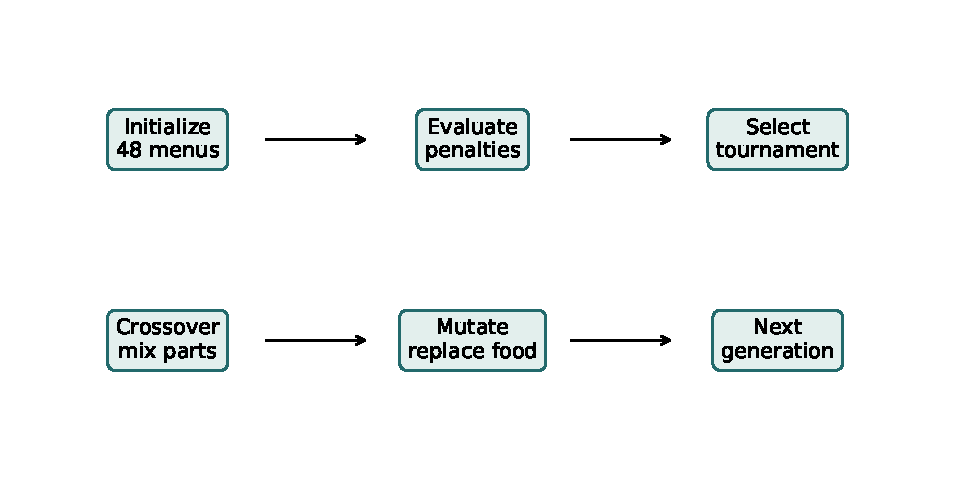
\includegraphics[width=\linewidth]{03/results/evolution_cycle.pdf}
\caption{弁当案の世代交代。選択・交叉・突然変異・評価を反復する。図は実装に対応した自作図。}
\end{figure}

選択・淘汰では、無作為に3案を選び、罰点が最も小さい案を親にするトーナメント選択を行う。
交叉では、親Aの前半と親Bの後半をつなぐ。
「ご飯と主菜の組合せ」と「副菜の組合せ」を異なる親から受け継ぐイメージである。
16区画の表現なので、交叉後も区画数は必ず16に保たれる。
突然変異では各区画を確率$1/16$で8種類から再抽選する。同じ食材も含むため、実際に食材が変わる確率は$7/128$である。この操作により親にない組合せを導入できる。
世代交代では48個の子を次世代とし、これまでの最良案を1個保存するエリート保存を加える。
最良案の罰点は悪化しないが、集団の多様性が維持される保証はない。

\subsection{コードで確かめる探索の改善}
人口48、60世代、乱数種0〜9の10試行を用いた。
初期集団を含め、各方式は2,928回の適合度評価を行う。
GAに加えて、交叉と選択だけで突然変異を除いた方式、毎回48案を独立に生成する無作為探索を比較した。
位置を入れ替えただけの弁当は同じ評価になるので、全ての食材個数ベクトル
$\sum_{j=0}^{7}c_j=16$を列挙して、最適値も独立に調べた。
その総数は$\binom{23}{7}=245,157$である。
遺伝子配列には同じ個数を表す重複があることを明記し、GAがこの全列挙より理論的に優れるとは主張しない。

\begin{table}[tb]\centering\small
\caption{10試行の最終罰点と厳密最適値への到達回数。全方式で評価回数は同一。}
\begin{tabular}{lrr}\toprule
方式 & 罰点の中央値 & 最適到達\\\midrule
GA & 0.23901 & 8/10\\
突然変異なし & 0.25494 & 2/10\\
無作為探索 & 0.30883 & 1/10\\\bottomrule
\end{tabular}\end{table}

全列挙による最適罰点は0.2390123457であり、食材個数の一例は
$(4,4,1,1,1,3,1,1)$であった。
表の通りGAの中央値はこの値と一致したが、2試行は最適値に届かなかった。
図の帯は乱数種間の四分位範囲であり、世代ごとの個体のばらつきではない。
突然変異を除くと、初期集団から失われた食材や配列部分を回復しにくくなり、早い段階で改善が止まる例が見られた。
この実験は、一つの評価関数において変異が役立つことを示す。
あらゆる最適化問題でGAが無作為探索に勝つという結論にはならない。

\begin{figure}[tb]\centering
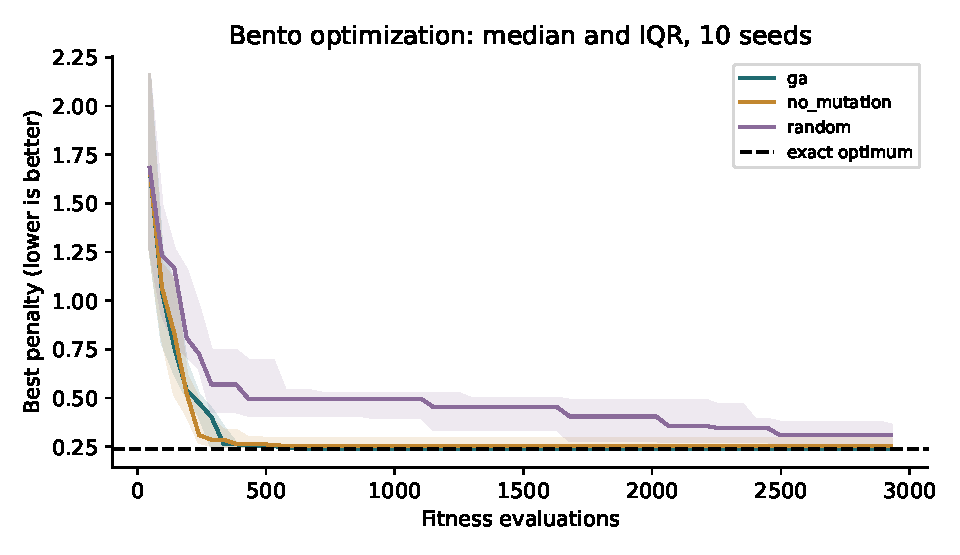
\includegraphics[width=\linewidth]{03/results/convergence.pdf}
\caption{最良罰点の中央値と四分位範囲。横軸を世代数でなく評価回数にそろえた。}
\end{figure}
\begin{figure}[tb]\centering
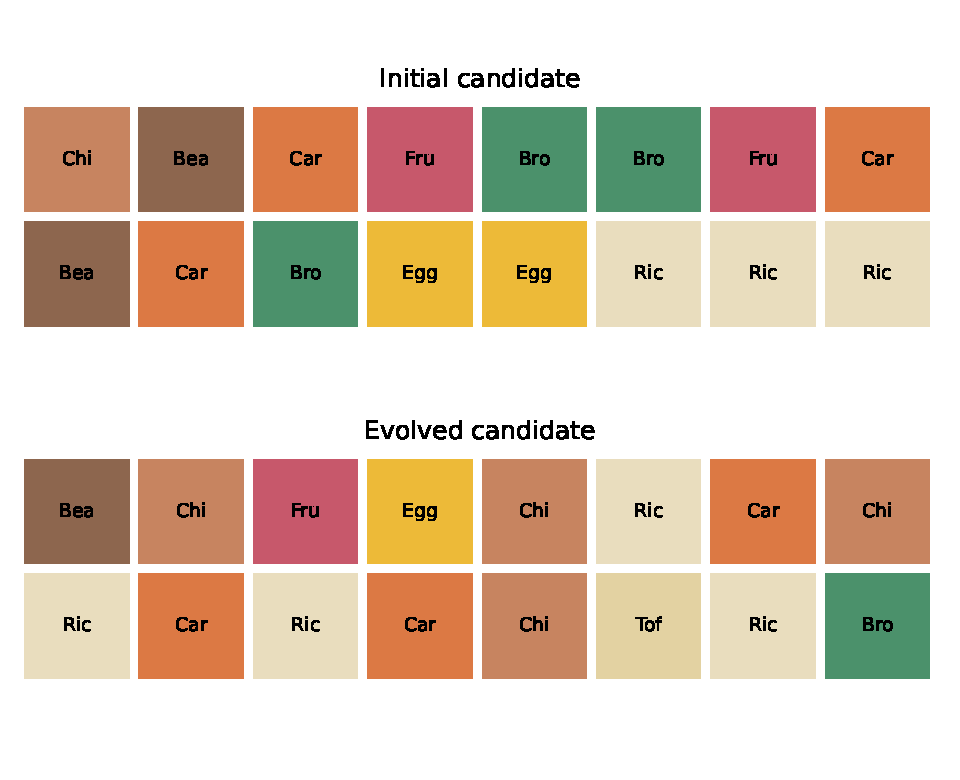
\includegraphics[width=\linewidth]{03/results/bento.pdf}
\caption{初期案と進化後の案。色は食材を表す。見た目の配置自体は今回の適合度に含めていない。}
\end{figure}

\subsection{応用例：細胞を集めるXenobotの形状設計}
課題の除外一覧にない応用として、Xenobotの形状設計を取り上げる。
これは既に工場で使われる製品というより、進化計算が実物の生物工学実験に接続した研究応用である。
研究者はカエル由来の細胞からなる小さな集合体を用い、周囲のばらばらの細胞を集める能力を調べた\cite{xenobot}。
進化的探索は、コンピュータ内で形状候補を評価し、細胞を集めやすい形を探すために使われた。
口の開いた形状を持つ集合体が、動きながら細胞をまとめるという機構は、「皿の上の細かい粒を、へらの形を変えて集める」と考えると理解しやすい。

\begin{figure}[tb]\centering
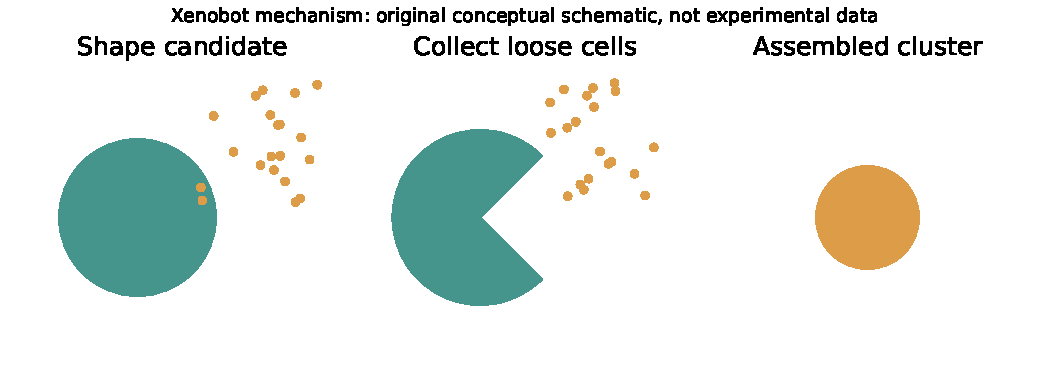
\includegraphics[width=\linewidth]{03/results/xenobot_schematic.pdf}
\caption{形状と細胞収集の関係を説明する独自の概念図。論文の顕微鏡画像や、本レポートによる生物実験の結果ではない。}
\end{figure}

弁当の例と対応させると、遺伝子は食材番号から形状のパラメータへ、適合度は栄養と予算から細胞を集めて次の集合体を生む能力へ置き換わる。
ここで「進化する」のは計算機内の設計候補であり、生物のDNAをGAが直接書き換えるという意味ではない。
研究チームの解説でもシミュレーションによる形状探索と実物の組立てが説明されている\cite{wyss}。
計算機の予測が実物でも成り立つかを調べる点が、この応用の重要な部分である。

この例が面白い理由は、制御プログラムだけでなく、\emph{形そのものが仕事をしやすくする}点にある。
弁当の最適値が評価式に依存したように、Xenobotでもシミュレータ、環境、測定する仕事を変えれば有利な形は変わりうる。
細胞の集まり方を正しくモデル化できなければ、計算上の高得点が実物の成功につながらない。
本レポートの弁当デモは進化計算の原理を説明するもので、Xenobotの物理や生物実験を再現したものではない。
\repolink{03}
